\documentclass[aspectratio=169, 10pt]{beamer}

% -----------------------------------------------------------------------------
% CONFIGURACIÓN DE IDIOMA Y CODIFICACIÓN
% -----------------------------------------------------------------------------
\usepackage[utf8]{inputenc}
\usepackage[T1]{fontenc}
\usepackage[spanish, es-tabla]{babel}

% -----------------------------------------------------------------------------
% PAQUETES GRÁFICOS Y MATEMÁTICOS (100% NATIVOS EN OVERLEAF)
% -----------------------------------------------------------------------------
\usepackage{amsmath, amssymb}
\usepackage{booktabs}
\usepackage{colortbl}
\usepackage{graphicx}
\usepackage{tikz}
\usetikzlibrary{shapes.geometric, arrows.meta, positioning, calc, backgrounds, fit}

% -----------------------------------------------------------------------------
% TEMA Y PALETA SOBRIA CORPORATIVA
% -----------------------------------------------------------------------------
\usetheme{Boadilla}
\useinnertheme{rectangles}

\definecolor{CINFBlue}{HTML}{122B4A}
\definecolor{CINFNavy}{HTML}{0F172A}
\definecolor{CINFRed}{HTML}{B4202A}
\definecolor{CINFGray}{HTML}{5B6573}

\definecolor{primaryBlue}{RGB}{15, 23, 42}
\definecolor{accentBlue}{RGB}{18, 43, 74}
\definecolor{alertRed}{RGB}{180, 32, 42}
\definecolor{successGreen}{RGB}{21, 122, 68}
\definecolor{darkSlate}{RGB}{30, 41, 59}
\definecolor{cardBg}{RGB}{248, 250, 252}

\setbeamercolor{palette primary}{bg=primaryBlue, fg=white}
\setbeamercolor{palette secondary}{bg=accentBlue, fg=white}
\setbeamercolor{palette tertiary}{bg=primaryBlue!90, fg=white}
\setbeamercolor{structure}{fg=accentBlue}
\setbeamercolor{titlelike}{fg=primaryBlue}
\setbeamercolor{frametitle}{bg=primaryBlue, fg=white}
\setbeamercolor{block title}{bg=accentBlue, fg=white}
\setbeamercolor{block body}{bg=cardBg, fg=darkSlate}
\setbeamercolor{block title alerted}{bg=alertRed, fg=white}
\setbeamercolor{block body alerted}{bg=alertRed!7, fg=darkSlate}
\setbeamercolor{block title example}{bg=successGreen, fg=white}
\setbeamercolor{block body example}{bg=successGreen!7, fg=darkSlate}

\setbeamertemplate{navigation symbols}{}
\setbeamertemplate{blocks}[rounded][shadow=false]
\setbeamertemplate{footline}{
  \leavevmode%
  \hbox{%
  \begin{beamercolorbox}[wd=.34\paperwidth,ht=2.4ex,dp=1ex,left,leftskip=1em]{author in head/foot}%
    \usebeamerfont{author in head/foot}\textbf{Felipe Vergara} · Ingeniería Civil Informática
  \end{beamercolorbox}%
  \begin{beamercolorbox}[wd=.48\paperwidth,ht=2.4ex,dp=1ex,center]{title in head/foot}%
    \usebeamerfont{title in head/foot}IoT Perimeter Guard · Detección de Anomalías mediante ML
  \end{beamercolorbox}%
  \begin{beamercolorbox}[wd=.18\paperwidth,ht=2.4ex,dp=1ex,right,rightskip=1em]{date in head/foot}%
    \insertframenumber{} / \inserttotalframenumber
  \end{beamercolorbox}}%
  \vskip0pt%
}

% -----------------------------------------------------------------------------
% METADATOS
% -----------------------------------------------------------------------------
\title[\textbf{IoT Perimeter Guard}]{\textbf{Sistema Centralizado de Detección de Anomalías en Redes IoT mediante Machine Learning}}
\subtitle{\textbf{Investigación Tecnológica Aplicada · Arquitectura, Validación Ciega 6/2/1 y Prototipo MVP}}
\author[\textbf{Felipe Vergara R.}]{\textbf{Felipe Nicolás Vergara Rodríguez}\\[1mm]\footnotesize Ingeniería Civil Informática}
\institute[\textbf{UNAB}]{\footnotesize Profesor Guía: \textbf{Nicolás Caselli Benavente}\\[1mm]Facultad de Ingeniería · Universidad Andrés Bello · Sede Viña del Mar}
\date[\textbf{Noviembre 2026}]{\small Noviembre de 2026}

\begin{document}

% -----------------------------------------------------------------------------
% SLIDE 1: PORTADA PROFESIONAL
% -----------------------------------------------------------------------------
\begin{frame}[plain]
  \begin{columns}[c]
    \begin{column}{0.74\textwidth}
      \titlepage
    \end{column}
    \begin{column}{0.23\textwidth}
      \centering
      \IfFileExists{logo_ici.png}{%
        
\includegraphics[width=0.92\linewidth]{logo_ici.png}\\[4mm]
      }{}
      \begin{beamercolorbox}[rounded=true,center,sep=2mm]{palette primary}
        \scriptsize \textbf{IoT Perimeter Guard}\\[1mm]
        \tiny Ciberseguridad · ML · Edge
      \end{beamercolorbox}
    \end{column}
  \end{columns}
\end{frame}

% -----------------------------------------------------------------------------
% SLIDE 2: HOJA DE RUTA
% -----------------------------------------------------------------------------
\begin{frame}{Estructura de la Presentación}
  \begin{columns}[T]
    \begin{column}{0.31\textwidth}
      \begin{block}{\textbf{1. Contexto y Método}}
        \footnotesize
        \begin{itemize}
          \item Problema en redes IoT
          \item Estado del arte (2018--2026)
          \item Objetivos y metas
          \item \textbf{Metodología Híbrida:}\\CRISP-DM / CRISP-ML(Q) + Scrum
        \end{itemize}
      \end{block}
    \end{column}
    \begin{column}{0.32\textwidth}
      \begin{block}{\textbf{2. Ingeniería y Pruebas}}
        \footnotesize
        \begin{itemize}
          \item Auditoría N-BaIoT (\texttt{HH\_jit})
          \item Arquitectura Doble Pipeline
          \item Defensa en 3 Anillos y Big-O
          \item Protocolo Ciego 6/2/1 (73 exp.)
          \item Ablaciones y caída Zero-Day
        \end{itemize}
      \end{block}
    \end{column}
    \begin{column}{0.31\textwidth}
      \begin{exampleblock}{\textbf{3. Impacto, Demo y Futuro}}
        \footnotesize
        \begin{itemize}
          \item Discusión crítica e impacto
          \item MVP, seguridad y Modo 24h
          \item Demostración interactiva
          \item Cumplimiento y plan 2027
        \end{itemize}
      \end{exampleblock}
    \end{column}
  \end{columns}
\end{frame}

% -----------------------------------------------------------------------------
% SLIDE 3: EL PROBLEMA + TOPOLOGÍA PERIMETRAL
% -----------------------------------------------------------------------------
\begin{frame}{El Problema: Vulnerabilidad Crítica en Redes IoT}
  \begin{columns}[c]
    \begin{column}{0.40\textwidth}
      \footnotesize
      \begin{alertblock}{\textbf{Limitación de Nodos IoT}}
        \begin{itemize}
          \item CPU y RAM mínimas; firmware cerrado sin antivirus.
          \item Reclutamiento DDoS (\textbf{Mirai} y \textbf{BASHLITE}).
        \end{itemize}
      \end{alertblock}
      \vspace{2mm}
      \begin{exampleblock}{\textbf{Solución: Defensa en Router}}
        \begin{itemize}
          \item \textbf{Cero carga en nodos:} Inspección perimetral en Gateway.
          \item \textbf{Metadatos de flujo:} Opera incluso con tráfico cifrado.
        \end{itemize}
      \end{exampleblock}
    \end{column}
    \begin{column}{0.56\textwidth}
      \centering
      \IfFileExists{fig_ppt_topologia_iot.png}{%
        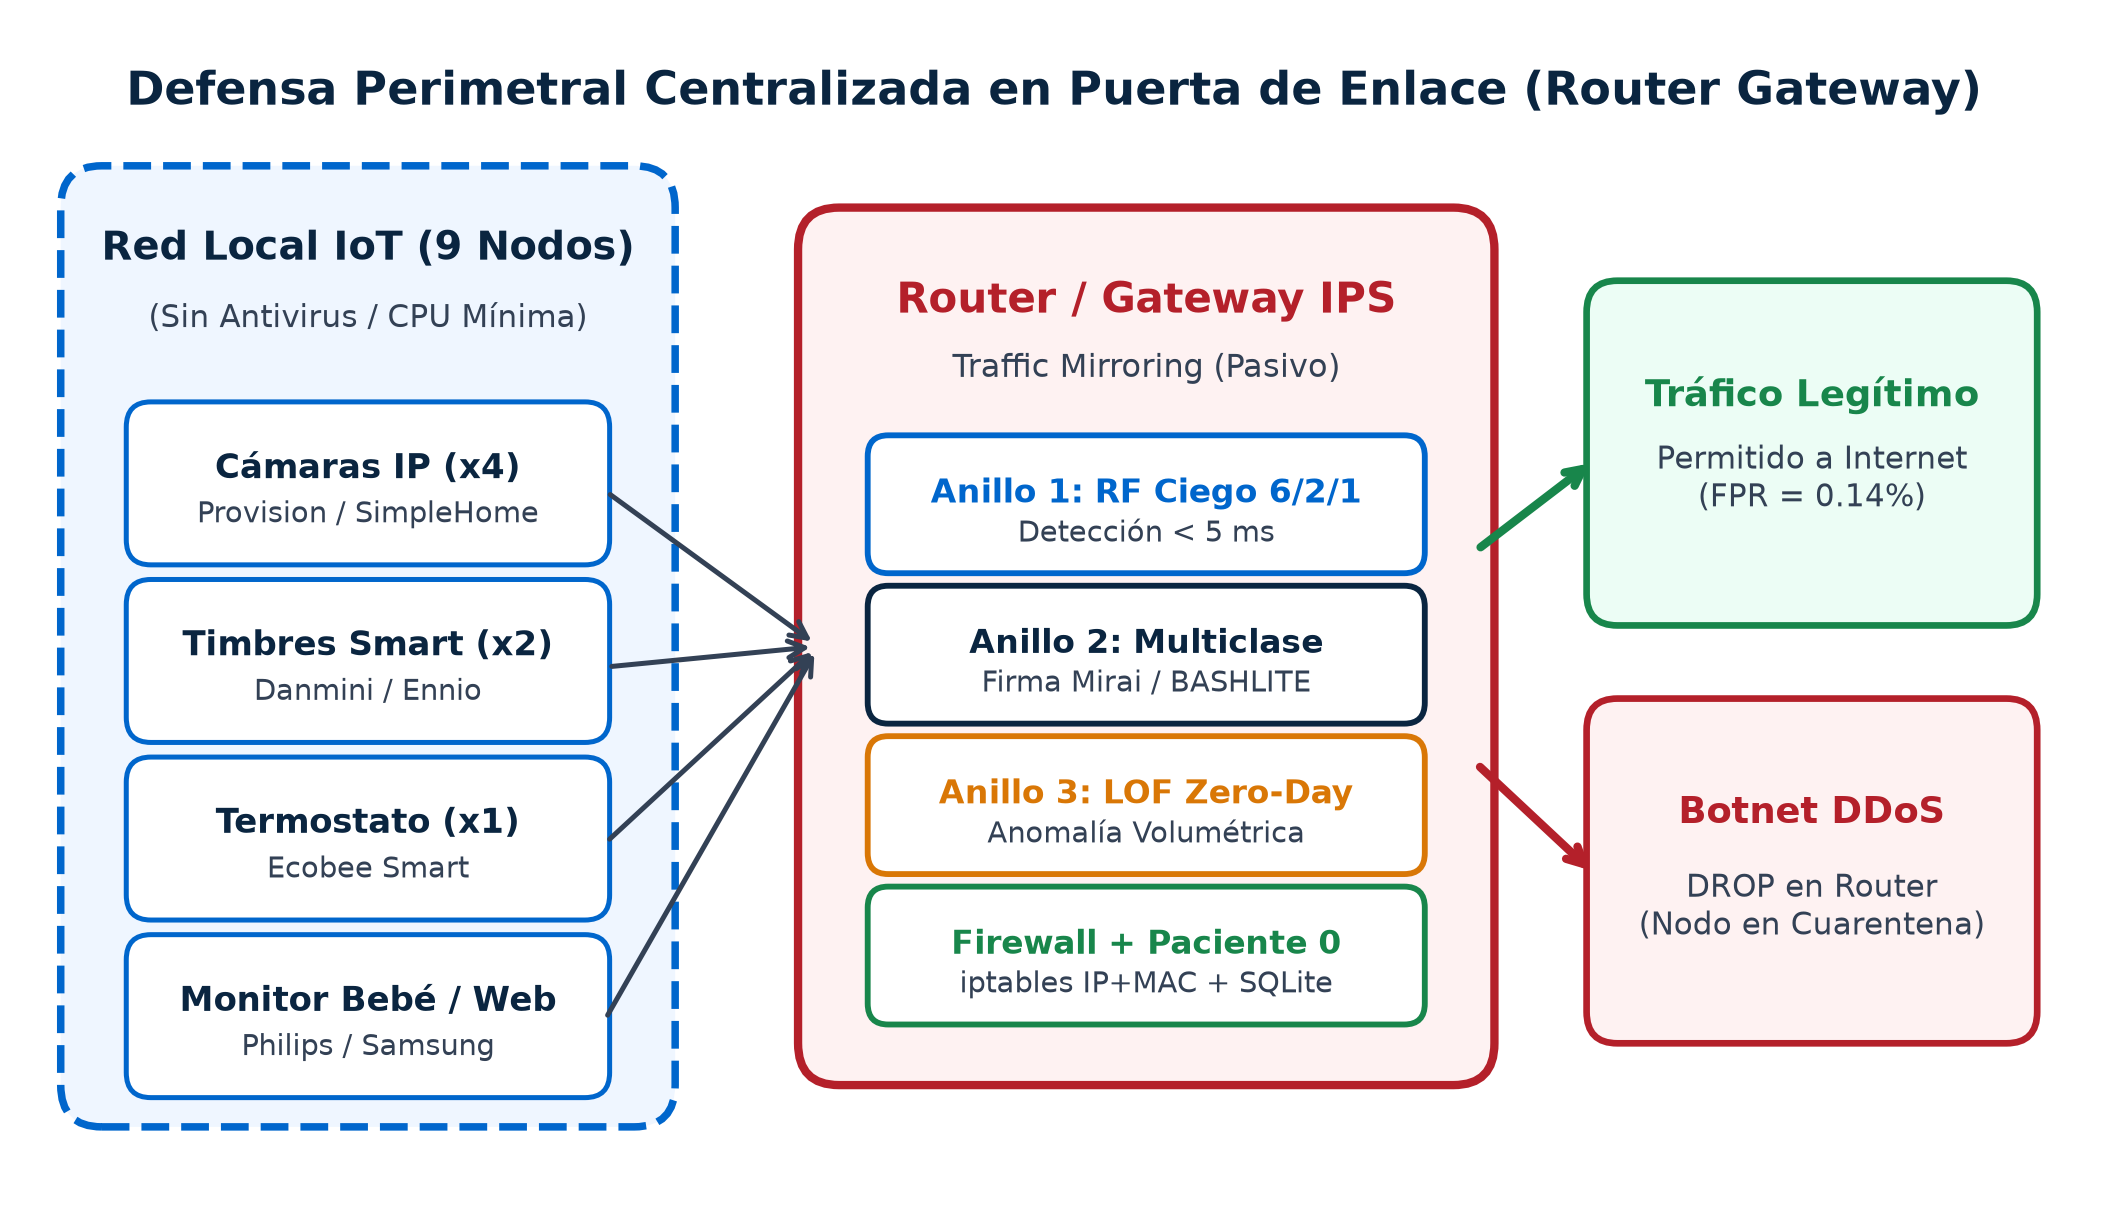
\includegraphics[width=\linewidth,height=0.72\textheight,keepaspectratio]{fig_ppt_topologia_iot.png}%
      }{}
    \end{column}
  \end{columns}
\end{frame}

% -----------------------------------------------------------------------------
% SLIDE 4: ESTADO DEL ARTE, BRECHA Y METAS
% -----------------------------------------------------------------------------
\begin{frame}{Estado del Arte (2018--2026) y Pregunta de Investigación}
  \begin{columns}[T]
    \begin{column}{0.56\textwidth}
      \begin{block}{\textbf{Brecha en la Literatura}}
        \footnotesize
        \begin{itemize}
          \item \textbf{Meidan et al. (2018):} 1 Autoencoder por equipo (\textit{no escala}).
          \item \textbf{Hossain (2023) / Naeem (2025):} $\sim$99\% en particiones estáticas.
          \item \textbf{Wardana (2024) / Bhilwarawala (2026):} Evidencian caídas severas al cambiar de dispositivo o dominio.
        \end{itemize}
      \end{block}
      \vspace{1mm}
      \begin{alertblock}{\textbf{Pregunta de Investigación}}
        \footnotesize
        ¿Cómo cambia el desempeño de clasificadores livianos al separar dispositivos (6/2/1) y excluir familias completas de botnets?
      \end{alertblock}
    \end{column}
    \begin{column}{0.39\textwidth}
      \begin{exampleblock}{\textbf{Metas Cuantitativas}}
        \footnotesize
        \begin{enumerate}
          \item \textbf{F1-Score:} $\ge 0{,}95$
          \item \textbf{Falsas Alarmas:} $\text{FPR} \le 1{,}0\%$
          \item \textbf{Latencia CPU:} $\le 10$ ms/vector
          \item \textbf{Explicabilidad:} Árboles + Z-Score
          \item \textbf{Calidad:} JWT, SHA-256, 25 tests
        \end{enumerate}
      \end{exampleblock}
    \end{column}
  \end{columns}
\end{frame}

% -----------------------------------------------------------------------------
% SLIDE 5: METODOLOGÍA HÍBRIDA CRISP-DM / CRISP-ML(Q) + SCRUM
% -----------------------------------------------------------------------------
\begin{frame}{Metodología Híbrida: CRISP-DM / CRISP-ML(Q) + Scrum}
  \centering
  \IfFileExists{fig_ppt_metodologia_hibrida.png}{%
    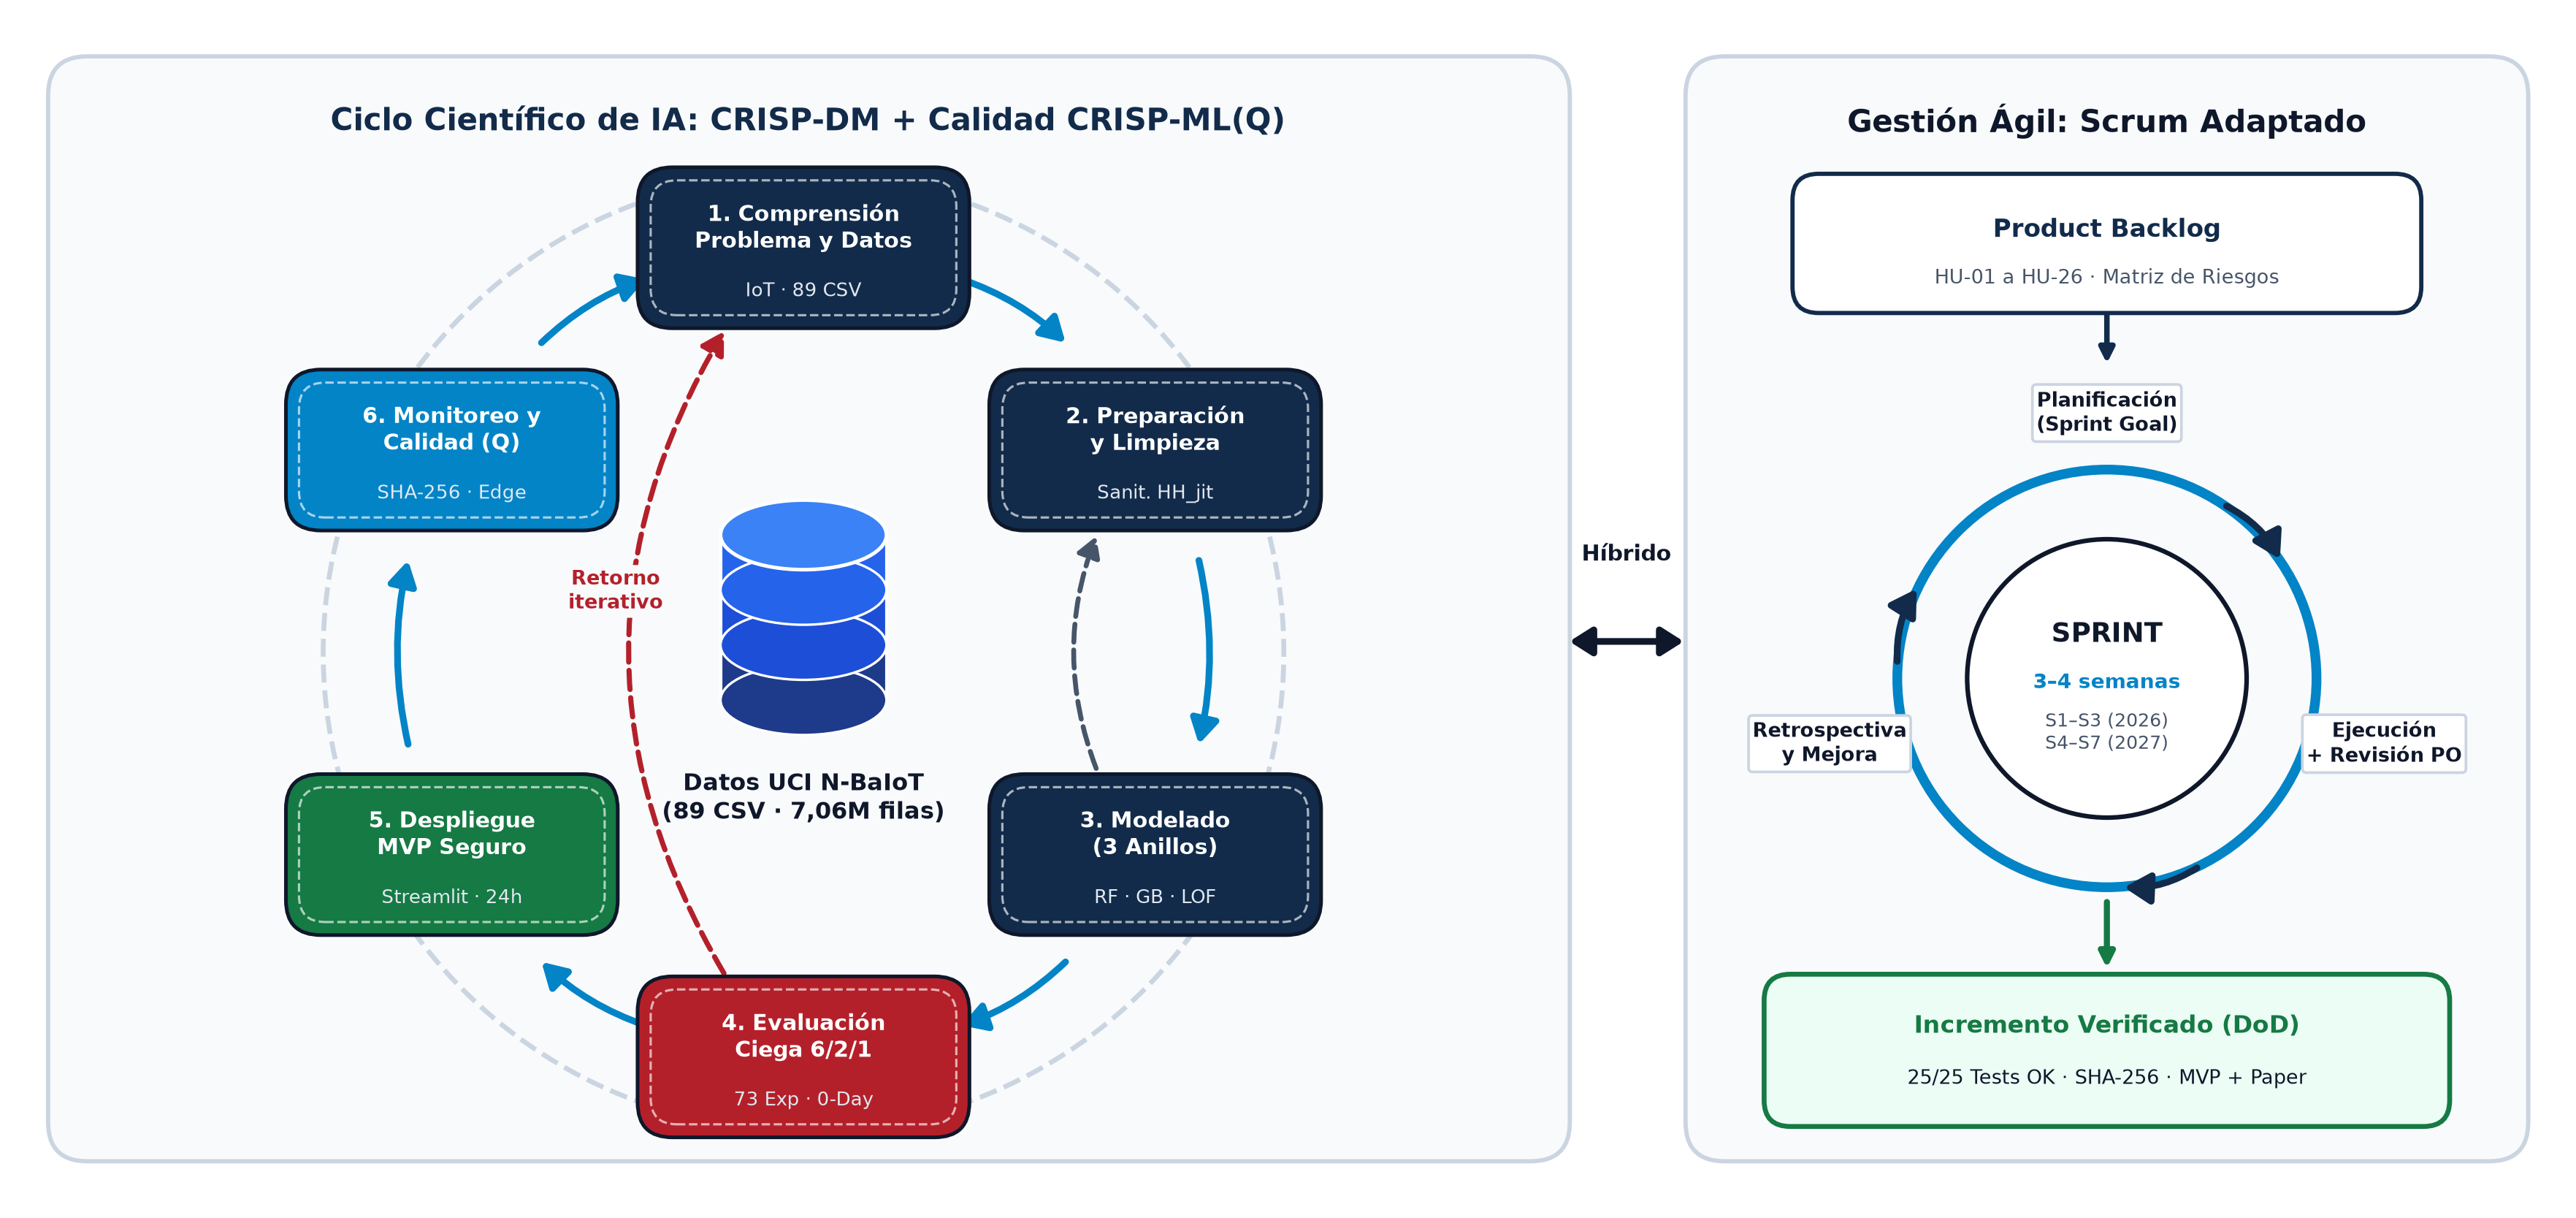
\includegraphics[width=0.96\textwidth,height=0.58\textheight,keepaspectratio]{fig_ppt_metodologia_hibrida.png}%
  }{%
    \fbox{\parbox[c][3cm][c]{0.85\textwidth}{\centering Ciclo circular CRISP-DM / CRISP-ML(Q) + Ciclo iterativo Scrum}}%
  }
  \vspace{2mm}
  \begin{columns}[T]
    \begin{column}{0.47\textwidth}
      \begin{block}{\textbf{Capa Científica (CRISP-DM + Calidad Q)}}
        \scriptsize Ciclo iterativo de 6 fases con retornos entre preparación, modelado y evaluación; audita fugas (\texttt{HH\_jit}) y robustez \textit{zero-day}.
      \end{block}
    \end{column}
    \begin{column}{0.47\textwidth}
      \begin{exampleblock}{\textbf{Capa Ágil (Scrum + Gestión de Riesgos)}}
        \scriptsize Sprints de 3--4 semanas (S1--S3 en 2026; S4--S7 en 2027), mitigando riesgos críticos con \textit{DoD} de 25 tests y \texttt{SHA-256}.
      \end{exampleblock}
    \end{column}
  \end{columns}
\end{frame}

% -----------------------------------------------------------------------------
% SLIDE 6: AUDITORÍA DE DATOS Y SANEAMIENTO HH_JIT
% -----------------------------------------------------------------------------
\begin{frame}{Auditoría de Datos y Saneamiento de Fuga (UCI N-BaIoT)}
  \begin{columns}[c]
    \begin{column}{0.40\textwidth}
      \footnotesize
      \begin{block}{\textbf{Dataset Auditado al 100\%}}
        \begin{itemize}
          \item \textbf{89 CSV:} 7.062.606 filas (\textbf{0 NaN/Inf}).
          \item \textbf{9 equipos reales} y \textbf{10 ataques} (Mirai / BASHLITE).
        \end{itemize}
      \end{block}
      \vspace{1.5mm}
      \begin{alertblock}{\textbf{Corrección de Fuga (\texttt{HH\_jit})}}
        \begin{itemize}
          \item \texttt{HH\_jit\_*\_mean} guardaba época Unix 2017 ($\sim 1{,}5\times 10^9$~s).
          \item Neutralizada a $0{,}0$; aprendizaje \textbf{100\% físico/volumétrico}.
        \end{itemize}
      \end{alertblock}
    \end{column}
    \begin{column}{0.56\textwidth}
      \centering
      \IfFileExists{fig_ppt_importancia_rf.png}{%
        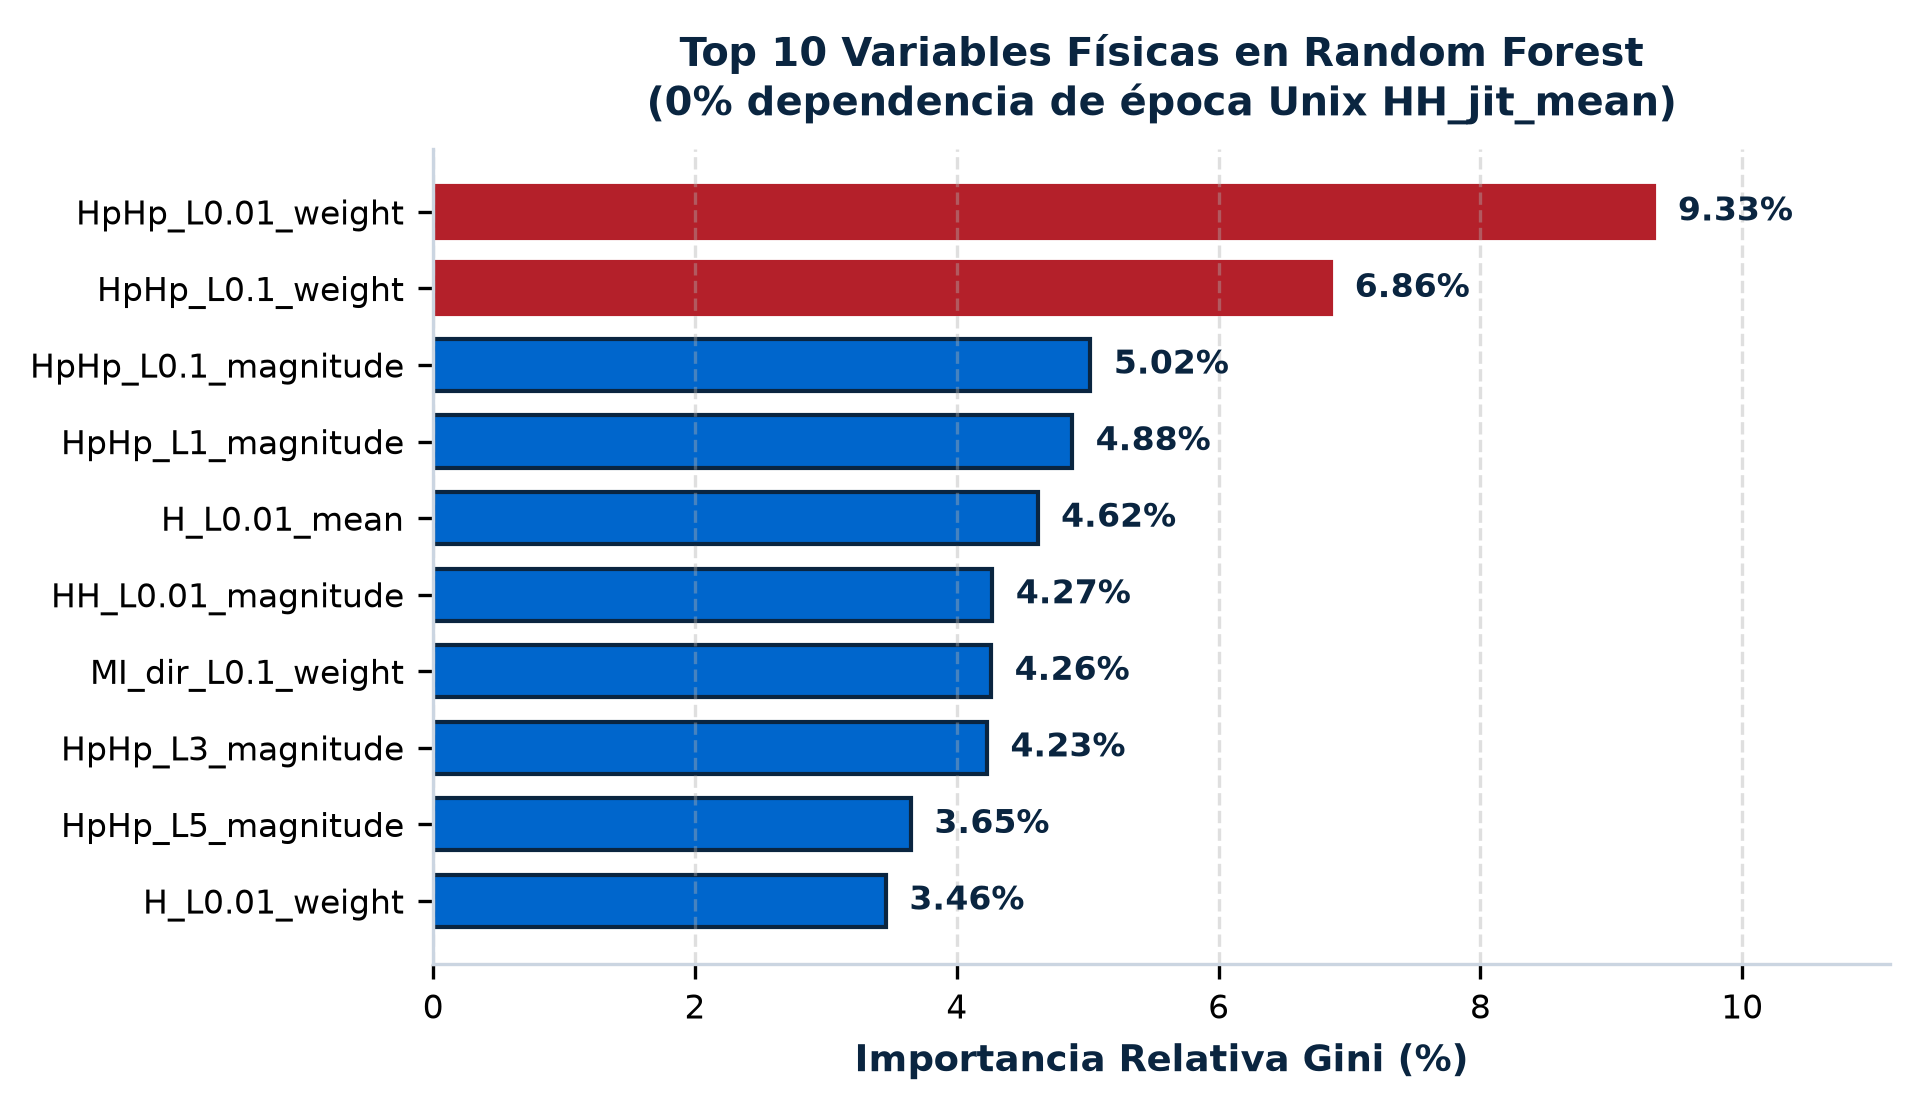
\includegraphics[width=\linewidth,height=0.72\textheight,keepaspectratio]{fig_ppt_importancia_rf.png}%
      }{}
    \end{column}
  \end{columns}
\end{frame}

% -----------------------------------------------------------------------------
% SLIDE 7: ARQUITECTURA DE DOBLE PIPELINE
% -----------------------------------------------------------------------------
\begin{frame}{Arquitectura General del Sistema: Doble Pipeline}
  \centering
  \resizebox{0.96\textwidth}{0.76\textheight}{%
  \begin{tikzpicture}[
    actor/.style={circle, draw=CINFNavy, fill=CINFNavy!5, very thick, minimum size=1.8cm, align=center, font=\small\bfseries\sffamily},
    sysbox/.style={rectangle, draw=CINFBlue, fill=CINFBlue!5, very thick, minimum width=3.2cm, minimum height=1.25cm, align=center, font=\small\bfseries\sffamily, rounded corners=3pt},
    db/.style={cylinder, draw=CINFNavy, fill=CINFNavy!10, very thick, minimum width=2.4cm, minimum height=1.25cm, align=center, font=\small\bfseries\sffamily, shape border rotate=90, aspect=0.25},
    modelbox/.style={rectangle, draw=CINFRed, fill=CINFRed!5, very thick, minimum width=3.4cm, minimum height=1.25cm, align=center, font=\small\bfseries\sffamily, rounded corners=6pt},
    arr/.style={-{Stealth[length=3mm]}, very thick, CINFGray!85!black},
    biarr/.style={{Stealth[length=3mm]}-{Stealth[length=3mm]}, very thick, CINFGray!85!black},
    lbl/.style={font=\scriptsize\bfseries\sffamily, text=CINFBlue!90!black, fill=white, inner sep=1.5pt, align=center},
    groupbox/.style={rectangle, draw=CINFGray, very thick, dashed, inner sep=10pt, rounded corners=5pt},
    grouplabel/.style={font=\normalsize\sffamily\bfseries, text=CINFNavy, anchor=north west}
  ]
  \node[actor]    (iot)         at (0, 2.6) {Catálogo N-BaIoT\\(9 dispositivos)};
  \node[sysbox]   (emulator)    at (4.6, 2.6) {Emulador / Inyector CSV\\+ Extractor O(1)};
  \node[actor]    (admin)       at (21.5, 2.6) {Operador /\\Analista};

  \node[sysbox, minimum width=3.8cm] (inference)   at (9.2, 0) {Motor IPS 3 Anillos\\(Binario Ciego + Multiclase + LOF)};
  \node[sysbox, minimum width=3.3cm] (firewall)    at (13.3, -2.0) {Firewall + Onboarding\\(iptables + Modo 24h)};
  \node[db]       (db_alerts)   at (18.0, -2.0) {Base de Datos SQLite\\(Alertas + Paciente Cero)};
  \node[sysbox, minimum width=3.4cm] (dashboard)   at (15.6, 0) {Consola Web MVP\\(IoT Perimeter Guard)};
  \node[sysbox, minimum width=3.3cm] (auth)        at (21.5, 0) {Control de Acceso\\(JWT + Rate Limit)};

  \draw[arr] (iot) -- (emulator) node[midway, lbl, above] {Trazas Test};
  \draw[arr] (emulator) -- (inference) node[pos=0.42, lbl, above, sloped] {Vectores 115 vars.};
  \draw[arr] (inference.south east) -- (firewall.north west) node[midway, lbl, below, sloped] {Alerta + Z-Score};
  \draw[arr] (firewall.north) -- ([xshift=-0.6cm]dashboard.south) node[midway, lbl, left] {Reglas IPS};
  \draw[arr] (firewall) -- (db_alerts) node[midway, lbl, below] {Registro};
  \draw[arr] (inference.east) -- (dashboard.west) node[midway, lbl, above] {Predicciones};
  \draw[arr] (db_alerts.north) -- ([xshift=0.7cm]dashboard.south) node[midway, lbl, right] {SQL / CSV};
  \draw[biarr] (dashboard) -- (auth) node[midway, lbl, above] {Sesión};
  \draw[biarr] (auth) -- (admin) node[pos=0.55, lbl, right] {Login JWT};

  \begin{scope}[on background layer]
    \coordinate (online_top) at (9.2, 1.05);
    \coordinate (online_bottom) at (9.2, -2.65);
    \node[groupbox, fill=CINFBlue!5, fit=(inference) (firewall) (db_alerts) (dashboard) (auth) (online_top) (online_bottom)] (online) {};
    \node[grouplabel] at (online.north west) {Pipeline Online: Consola Operativa MVP (Sistema IPS Centralizado de 3 Anillos)};
  \end{scope}

  \node[db]       (dataset)     at (0, -6.2) {Dataset N-BaIoT\\(89 CSV / 7M filas)};
  \node[sysbox]   (preproc_off) at (4.6, -6.2) {Ingeniería de Datos\\(Sanitización HH\_jit)};
  \node[sysbox]   (train)       at (9.2, -6.2) {Entrenamiento ML\\(RF, GB, LR, SVM, LOF)};
  \node[sysbox]   (eval)        at (9.2, -4.3) {Validación Científica\\(LODO 8/1 y Riguroso 6/2/1)};
  \node[modelbox, minimum width=3.8cm] (registry) at (15.6, -6.2) {Artefactos .pkl y Folds Ciegos\\(Manifiesto SHA-256)};

  \draw[arr] (dataset) -- (preproc_off) node[midway, lbl, above] {Batch};
  \draw[arr] (preproc_off) -- (train) node[midway, lbl, above] {Bloques};
  \draw[biarr] (train) -- (eval) node[midway, lbl, right] {73 Exp.};
  \draw[arr] (train) -- (registry) node[midway, lbl, above] {Serialización};
  \draw[arr] (eval.east) -| (registry.north) node[pos=0.25, lbl, above] {Candidatos 6/2/1 y Métricas};

  \begin{scope}[on background layer]
    \coordinate (offline_top) at (9.2, -3.35);
    \node[groupbox, fill=CINFGray!5, fit=(dataset) (preproc_off) (train) (eval) (registry) (offline_top)] (offline) {};
    \node[grouplabel] at (offline.north west) {Pipeline Offline: Ciclo CRISP-DM / CRISP-ML(Q) e Investigación};
  \end{scope}

  \draw[arr, dashed, CINFRed!80!black] ([xshift=-0.5cm]registry.north) -- (15.1, -3.0) -- (9.7, -3.0) node[midway, lbl, above] {Modelos + Folds Ciegos (SHA-256)} -- ([xshift=0.5cm]inference.south);
  \draw[arr, dashed, CINFNavy!60] (preproc_off.north) -- (4.6, -3.0) -- (8.7, -3.0) node[midway, lbl, above] {Scalers} -- ([xshift=-0.5cm]inference.south);
  \end{tikzpicture}
  }%
\end{frame}

% -----------------------------------------------------------------------------
% SLIDE 8: DEFENSA EN 3 ANILLOS Y COMPLEJIDAD
% -----------------------------------------------------------------------------
\begin{frame}{Defensa en 3 Anillos y Eficiencia Algorítmica}
  \begin{columns}[T]
    \begin{column}{0.31\textwidth}
      \begin{block}{\textbf{Anillo 1: Binario Ciego}}
        \footnotesize
        \begin{itemize}
          \item \textbf{Random Forest} (6/2/1).
          \item Inferencia: $O(k \cdot \text{prof.})$.
          \item \textbf{5,28 ms} CPU · 0,3--2,5 MB.
        \end{itemize}
      \end{block}
    \end{column}
    \begin{column}{0.32\textwidth}
      \begin{block}{\textbf{Anillo 2: Firma Botnet}}
        \footnotesize
        \begin{itemize}
          \item \textbf{Multiclase} (10 ataques).
          \item Precisión canónica: \textbf{91,76\%}.
          \item Identifica Mirai / BASHLITE sin etiquetas externas.
        \end{itemize}
      \end{block}
    \end{column}
    \begin{column}{0.31\textwidth}
      \begin{alertblock}{\textbf{Anillo 3: Zero-Day}}
        \footnotesize
        \begin{itemize}
          \item \textbf{LocalOutlierFactor (LOF)}.
          \item Entrenado \textbf{100\% benigno}.
          \item Recall sin ver ataques: \textbf{75,60\%}.
        \end{itemize}
      \end{alertblock}
    \end{column}
  \end{columns}
  \vspace{3mm}
  \begin{exampleblock}{\textbf{¿Por qué Machine Learning Clásico frente a Deep Learning?}}
    \footnotesize Inferencia bajo $10$~ms en CPU convencional sin GPU, tamaño compacto ($<2{,}5$~MB), menor tasa de falsos positivos frente a modelos lineales ($O(d)$) y explicabilidad nativa (\textit{Feature Importance} + Z-Score).
  \end{exampleblock}
\end{frame}

% -----------------------------------------------------------------------------
% SLIDE 9: PROTOCOLO RIGUROSO 6/2/1
% -----------------------------------------------------------------------------
\begin{frame}{Protocolo Riguroso 6/2/1: 9 Folds en Rotación Ciega}
  \begin{columns}[c]
    \begin{column}{0.40\textwidth}
      \footnotesize
      \begin{block}{\textbf{Rotación de 9 Modelos Ciegos}}
        \begin{itemize}
          \item \textbf{6 Disp.} $\to$ Ajuste ($10\%, 30\%$).
          \item \textbf{2 Disp.} $\to$ Calibración $\text{FPR}\le 0{,}1\%$ ($50\%, 65\%$).
          \item \textbf{1 Disp.} $\to$ \textbf{Test 100\% Ciego} ($80\%, 95\%$).
          \item \textbf{Total:} 73 exp. con firma \texttt{SHA-256}.
        \end{itemize}
      \end{block}
      \vspace{1.5mm}
      \begin{exampleblock}{\textbf{Enrutamiento en Vivo}}
        Al evaluar \textbf{Disp. $X$} se activa \textbf{\texttt{device\_X\_rf}} (\textbf{0\% visto} en ajuste y calibración).
      \end{exampleblock}
    \end{column}
    \begin{column}{0.56\textwidth}
      \centering
      \IfFileExists{fig_ppt_protocolo_621.png}{%
        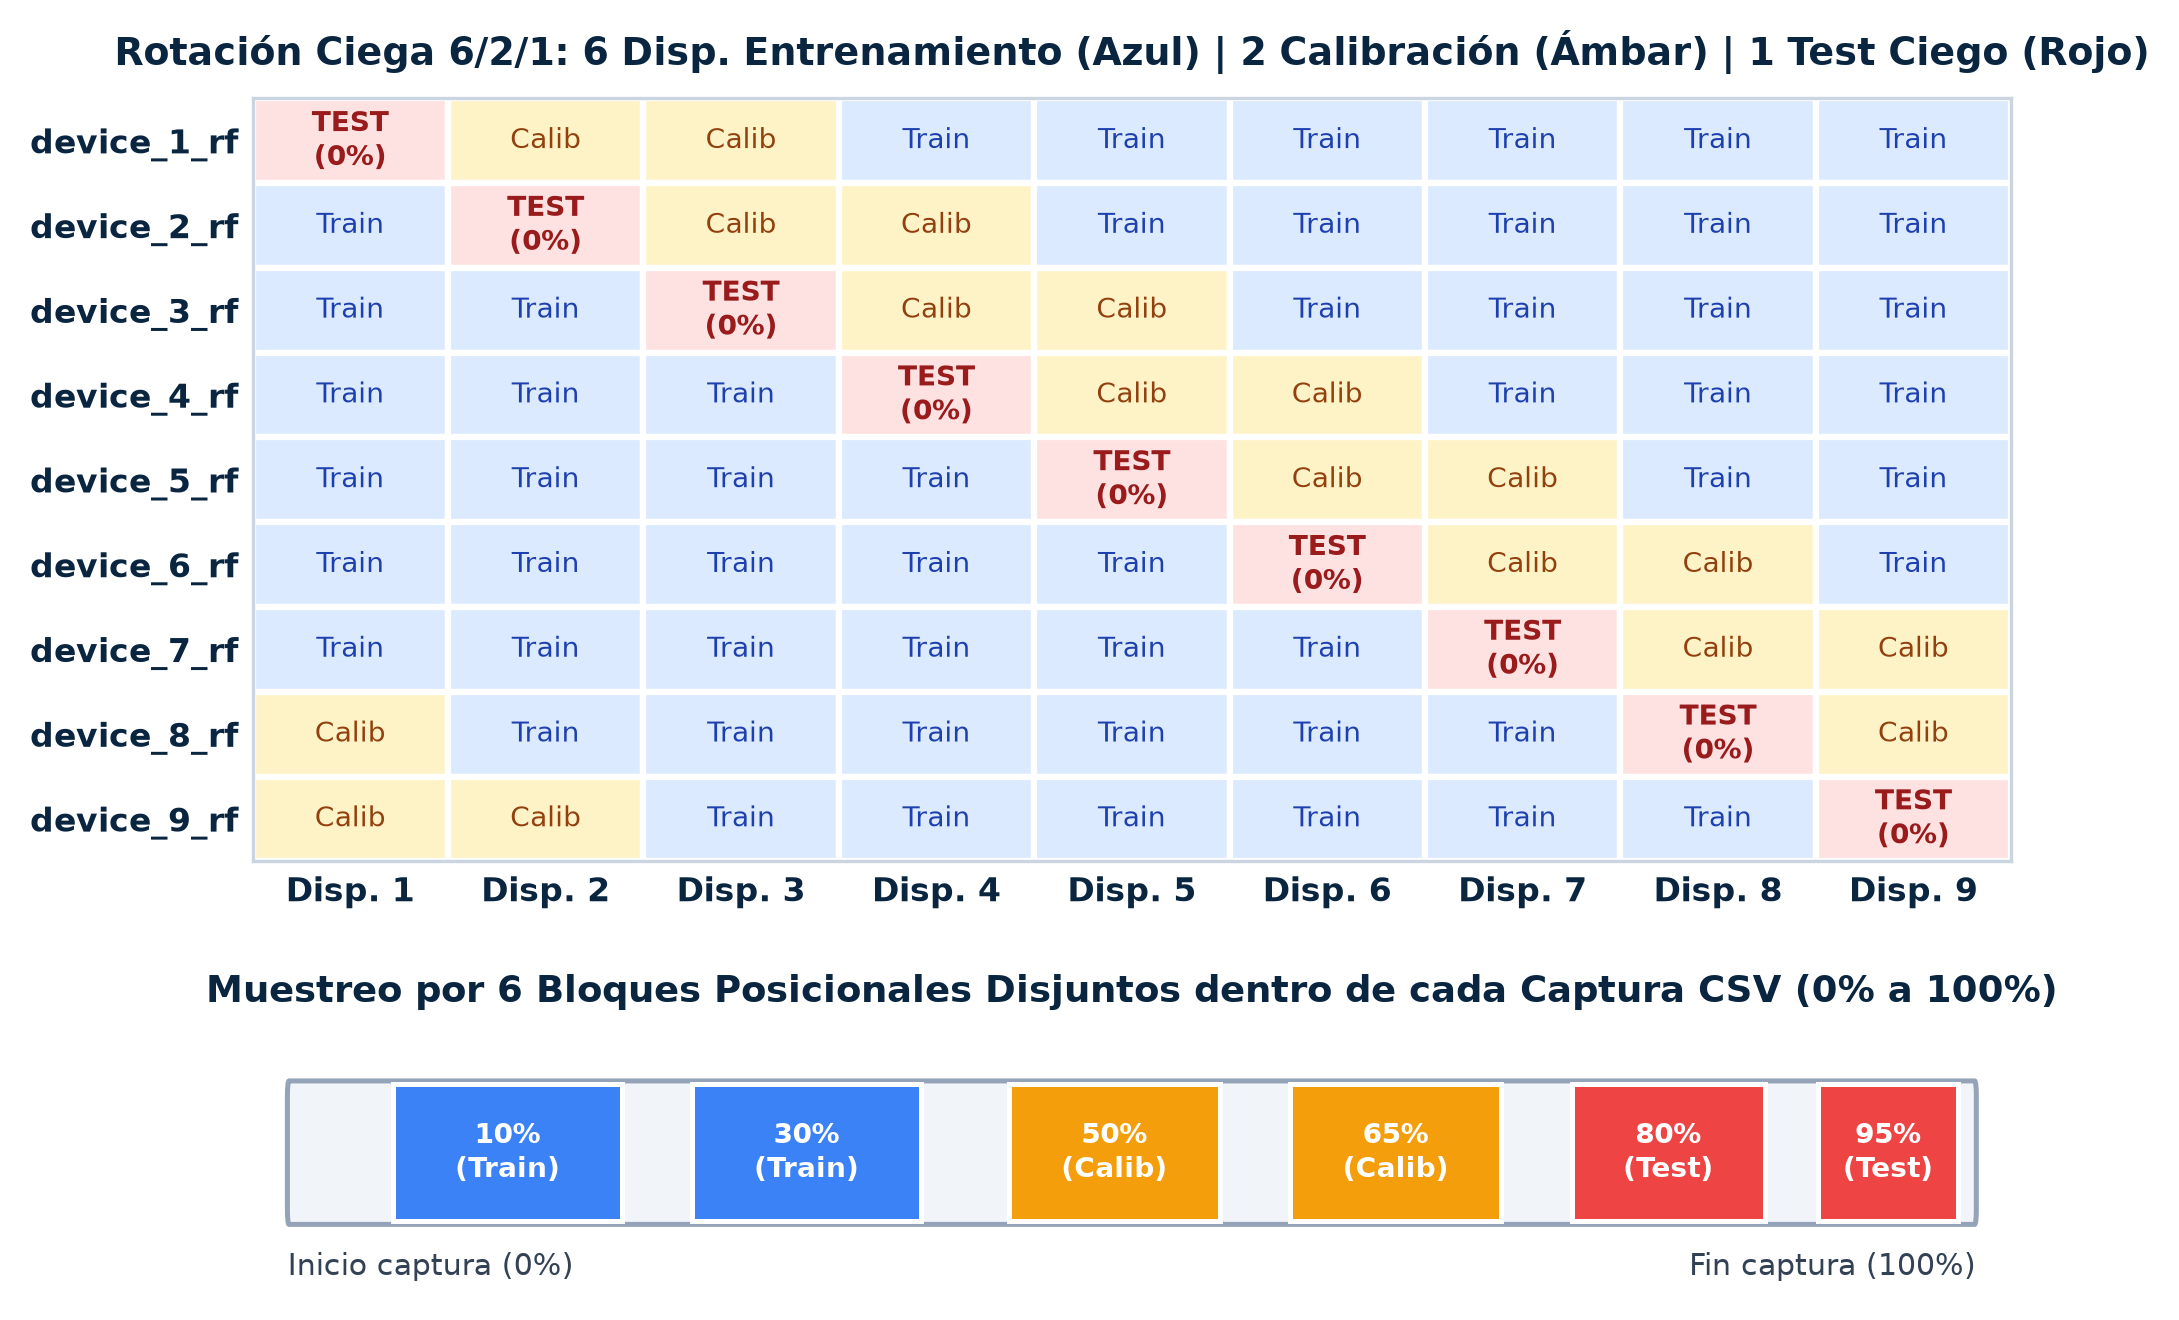
\includegraphics[width=\linewidth,height=0.73\textheight,keepaspectratio]{fig_ppt_protocolo_621.png}%
      }{}
    \end{column}
  \end{columns}
\end{frame}

% -----------------------------------------------------------------------------
% SLIDE 10: RESULTADOS CONSOLIDADOS Y ABLACIÓN
% -----------------------------------------------------------------------------
\begin{frame}{Resultados Consolidados: Línea Base, 6/2/1 y Ablación}
  \begin{columns}[T]
    \begin{column}{0.52\textwidth}
      \footnotesize\textbf{Evaluación en Dispositivo Excluido (9 Folds 6/2/1):}\\[2mm]
      \resizebox{\linewidth}{!}{%
      \begin{tabular}{llccc}
        \toprule
        \textbf{Modelo} & \textbf{Umbral} & \textbf{F1 Medio} & \textbf{FPR} & \textbf{Min.\ Rec.} \\
        \midrule
        \texttt{Dummy} (Ref.\ Hist.) & Control & 0,0000 & 0,00\% & 0,00\% \\
        \midrule
        Reg.\ Logística & Ajustado & \textbf{0,8007} & 0,04\% & \textbf{22,62\%} \\
        Grad.\ Boosting & Ajustado & \textbf{0,9452} & 2,95\% & \textbf{60,00\%} \\
        \textbf{Random Forest} & \textbf{Ajustado} & \textbf{0,9995} & \textbf{0,14\%} & \textbf{99,95\%} \\
        \bottomrule
      \end{tabular}
      }%
      \vspace{3mm}
      \begin{block}{\textbf{Latencia Unitaria CPU (Meta $\le 10$ ms)}}
        \scriptsize LR: \textbf{0,13 ms} · GB: \textbf{1,03 ms} · SVM: \textbf{1,39 ms} · RF: \textbf{5,28 ms}.
      \end{block}
    \end{column}
    \begin{column}{0.43\textwidth}
      \footnotesize\textbf{Ablación de Variables (Random Forest):}\\[2mm]
      \resizebox{\linewidth}{!}{%
      \begin{tabular}{lcc}
        \toprule
        \textbf{Representación} & \textbf{F1 Medio} & \textbf{Min.\ Rec.} \\
        \midrule
        \textbf{Sanitizada (105 v.)} & \textbf{0,9995} & \textbf{99,95\%} \\
        Jitter crudo (fuga) & 0,9988 & 99,98\% \\
        Sin pesos (\texttt{weight}) & \textbf{0,8919} & \textbf{69,00\%} \\
        Sin ventanas lentas & \textbf{0,8583} & \textbf{29,25\%} \\
        \bottomrule
      \end{tabular}
      }%
      \vspace{3mm}
      \begin{alertblock}{\textbf{Hallazgo Físico Clave}}
        \scriptsize Sin ventanas lentas ($\lambda=0{,}01, 0{,}1$) el peor recall cae a \textbf{29,25\%}.
      \end{alertblock}
    \end{column}
  \end{columns}
\end{frame}

% -----------------------------------------------------------------------------
% SLIDE 11: PRUEBA DE FUEGO ZERO-DAY
% -----------------------------------------------------------------------------
\begin{frame}{Prueba de Fuego: Exclusión Total de Familias (Zero-Day)}
  \begin{columns}[c]
    \begin{column}{0.40\textwidth}
      \footnotesize
      \begin{alertblock}{\textbf{Caída Real (16 Escenarios)}}
        \begin{itemize}
          \item \textbf{Sin Mirai (Disp. 4):} Recall \textbf{39,90\%} ($F1=0{,}5702$; 1.202 FN).
          \item \textbf{Sin BASHLITE (Disp. 6):} Recall \textbf{48,55\%} ($F1=0{,}6537$; 1.029 FN).
        \end{itemize}
      \end{alertblock}
      \vspace{1.5mm}
      \begin{exampleblock}{\textbf{Qué Demuestra este Hallazgo}}
        \begin{itemize}
          \item \textbf{Cero Fuga de Código:} Si hubiera trampa, daría $99\%$ igual.
          \item \textbf{Justifica Anillo 3 (LOF):} Respaldo volumétrico sin firmas.
        \end{itemize}
      \end{exampleblock}
    \end{column}
    \begin{column}{0.56\textwidth}
      \centering
      \IfFileExists{fig_ppt_zeroday_caida.png}{%
        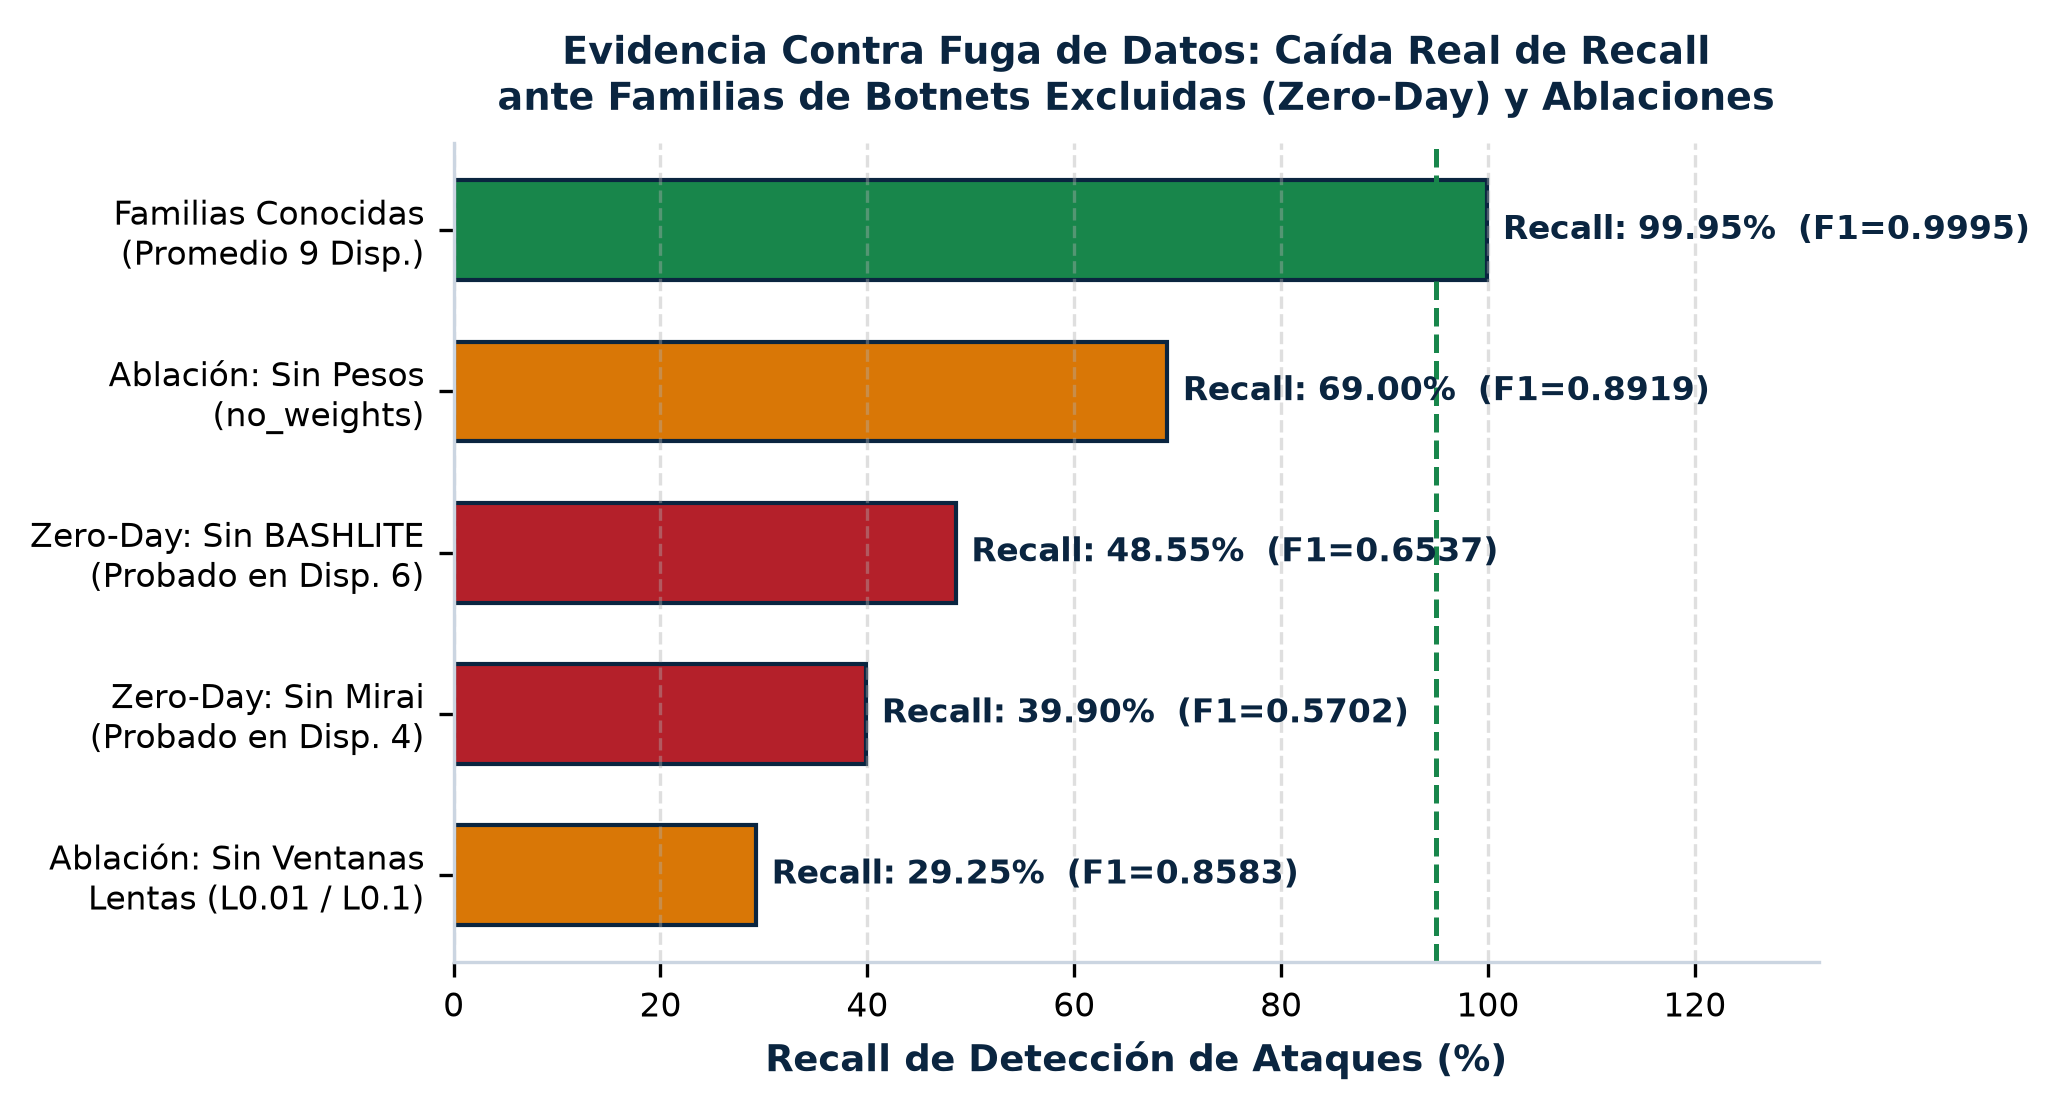
\includegraphics[width=\linewidth,height=0.73\textheight,keepaspectratio]{fig_ppt_zeroday_caida.png}%
      }{}
    \end{column}
  \end{columns}
\end{frame}

% -----------------------------------------------------------------------------
% SLIDE 12: DISCUSIÓN CRÍTICA E IMPACTO
% -----------------------------------------------------------------------------
\begin{frame}{Discusión Crítica, Contraste e Impacto}
  \begin{columns}[T]
    \begin{column}{0.47\textwidth}
      \begin{block}{\textbf{Contraste con Literatura}}
        \footnotesize
        \begin{itemize}
          \item \textbf{Meidan (2018) / Hossain (2023):} Altas métricas en familias conocidas no garantizan transferencia \textit{zero-day}.
          \item \textbf{Wardana (2024) / Bhilwarawala (2026):} Confirmamos la brecha \textit{cross-domain} bajo protocolo saneado 6/2/1.
        \end{itemize}
      \end{block}
      \vspace{1.5mm}
      \begin{exampleblock}{\textbf{Impacto: Usuarios, Procesos y Sociedad}}
        \footnotesize
        \begin{itemize}
          \item Ciberseguridad proactiva local y privada (sin nube ni lectura de \textit{payload}).
          \item Evita reclutamiento de hogares en botnets DDoS contra servicios críticos.
        \end{itemize}
      \end{exampleblock}
    \end{column}
    \begin{column}{0.47\textwidth}
      \begin{alertblock}{\textbf{Limitaciones y Amenazas a la Validez}}
        \footnotesize
        \begin{itemize}
          \item \textbf{Temporalidad:} Dataset N-BaIoT capturado en 2018 (sin QUIC/HTTP3).
          \item \textbf{Prevalencia:} Bloques balanceados no miden falsas alarmas diarias reales.
          \item \textbf{Operación:} Replay CSV; certificación numérica del extractor $O(1)$ y bloqueo físico en OpenWrt quedan para 2027.
        \end{itemize}
      \end{alertblock}
    \end{column}
  \end{columns}
\end{frame}

% -----------------------------------------------------------------------------
% SLIDE 13: CONSOLA MVP, CIBERSEGURIDAD Y MODO 24H
% -----------------------------------------------------------------------------
\begin{frame}{Prototipo MVP (\textit{IoT Perimeter Guard}), Seguridad y Modo 24h}
  \begin{columns}[c]
    \begin{column}{0.40\textwidth}
      \scriptsize
      \begin{block}{\textbf{Defensa en Profundidad y UX}}
        \begin{itemize}
          \item \textbf{JWT \texttt{HS256}} + \textit{rate limiting} fuerza bruta.
          \item \textbf{SHA-256} previo a cargar modelos + SQLite parametrizado (exportación CSV).
          \item \textbf{Firewall IP+MAC} + Whitelist (\texttt{192.168.1.1}).
          \item Traductor humano de Z-Score y \textbf{25/25 tests OK}.
        \end{itemize}
      \end{block}
      \vspace{1.5mm}
      \begin{exampleblock}{\textbf{Nuevos Equipos e Invitados}}
        \begin{itemize}
          \item \textbf{Modo Aprendizaje 24h:} Auto-calibra umbral personal ($Q_{99{,}5}+0{,}05$) sin bloqueos prematuros.
          \item \textbf{Modo Social:} Ante ráfagas ($\ge 3$ invitados), evita desconectar el Wi-Fi por falsas alarmas.
        \end{itemize}
      \end{exampleblock}
    \end{column}
    \begin{column}{0.56\textwidth}
      \centering
      \IfFileExists{dashboard_funcionando.png}{%
        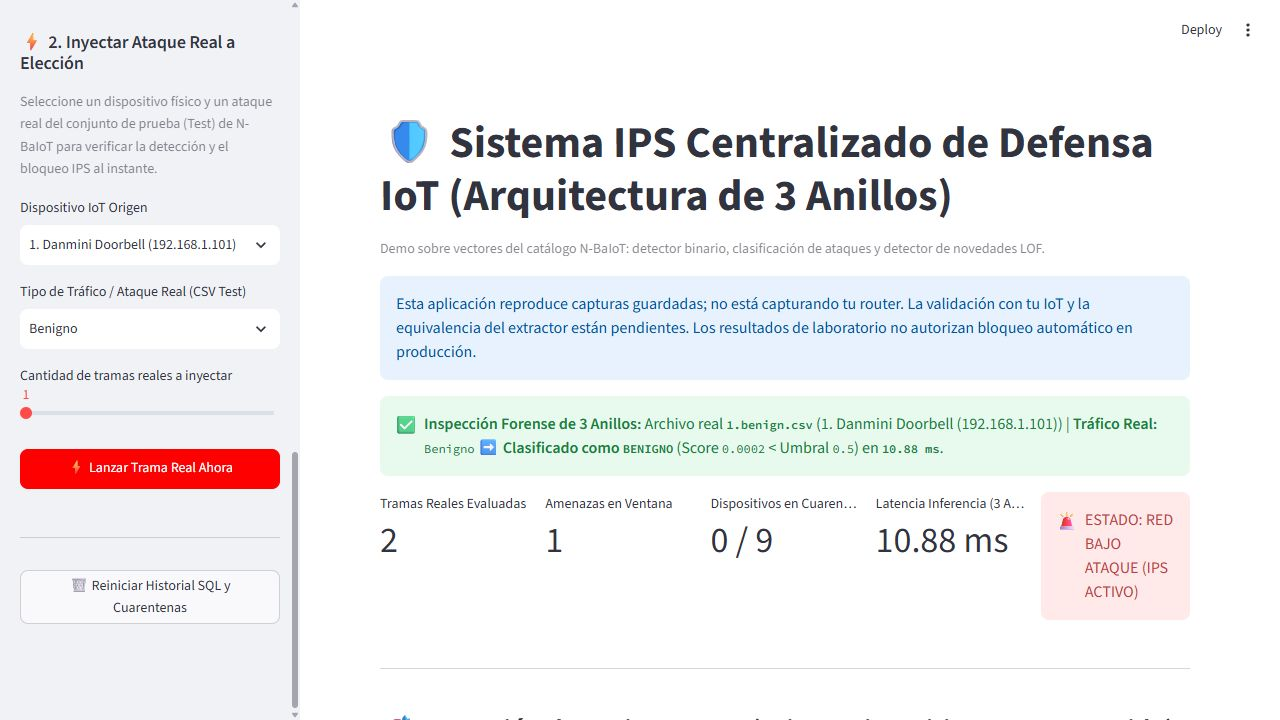
\includegraphics[width=\linewidth,height=0.73\textheight,keepaspectratio]{dashboard_funcionando.png}%
      }{}
    \end{column}
  \end{columns}
\end{frame}

% -----------------------------------------------------------------------------
% SLIDE 14: PASE A DEMOSTRACIÓN EN VIVO
% -----------------------------------------------------------------------------
\begin{frame}{Demostración Interactiva en Vivo}
  \centering
  \vspace{2mm}
  \begin{beamercolorbox}[rounded=true,center,sep=3.5mm,wd=0.84\textwidth]{palette primary}
    {\Large \textbf{PASE A DEMOSTRACIÓN EN VIVO (\textit{IoT Perimeter Guard})}}\\[2mm]
    {\small Consola Local en Ejecución: \texttt{http://localhost:8501}}
  \end{beamercolorbox}
  \vspace{5mm}
  \begin{columns}[T]
    \begin{column}{0.23\textwidth}
      \centering
      \textbf{1. Acceso y Normal}\\
      \scriptsize Login JWT + Escenario \textit{Día normal en casa} (9/9 verde).
    \end{column}
    \begin{column}{0.24\textwidth}
      \centering
      \textbf{2. Ataque Ciego 6/2/1}\\
      \scriptsize Dispositivo $X$ evaluado por \texttt{device\_X\_rf} (0\% visto) + diagnóstico simple.
    \end{column}
    \begin{column}{0.25\textwidth}
      \centering
      \textbf{3. Modo 24h e Invitados}\\
      \scriptsize Cámara nueva auto-calibrada + Cumpleaños (+9 invitados).
    \end{column}
    \begin{column}{0.23\textwidth}
      \centering
      \textbf{4. Forense y SHA-256}\\
      \scriptsize Paciente Cero, \texttt{iptables}, CSV y hashes verificados.
    \end{column}
  \end{columns}
\end{frame}

% -----------------------------------------------------------------------------
% SLIDE 15: CUMPLIMIENTO 2026 Y CONTINUIDAD 2027
% -----------------------------------------------------------------------------
\begin{frame}{Cumplimiento de Objetivos 2026 y Continuidad 2027}
  \begin{columns}[T]
    \begin{column}{0.49\textwidth}
      \begin{exampleblock}{\textbf{Logros Consolidados 2026 (Sprints 1--3: 100\%)}}
        \footnotesize
        \begin{itemize}
          \item \textbf{OE1--OE2:} Estado del arte (6 fuentes) y 7,06M filas saneadas sin época Unix.
          \item \textbf{OE3--OE4:} 5 modelos vs \texttt{Dummy} + 73 exp.\ ciegos 6/2/1 + 16 Zero-Day.
          \item \textbf{OE5--OE6:} MVP minimalista, Modo 24h/Invitados, \textbf{25/25 tests}, Paper, Póster A0 y Portafolio (10 evidencias).
        \end{itemize}
      \end{exampleblock}
    \end{column}
    \begin{column}{0.46\textwidth}
      \begin{block}{\textbf{Continuidad Experimental 2027 (Sprints 4--7)}}
        \vspace{1mm}
        \resizebox{\linewidth}{!}{%
        \begin{tabular}{lll}
          \toprule
          \textbf{Etapa / Sprint} & \textbf{Objetivo Técnico} & \textbf{Periodo} \\
          \midrule
          Etapa 8 (S4) & Despliegue \textit{Edge} (Raspberry Pi) & Mar--Abr \\
          Etapa 9 (S5) & Extractor $O(1)$ en \texttt{.pcap} en vivo & Abr--May \\
          Etapa 10 (S6) & FPR real hogar + OpenWrt & May--Jun \\
          Etapa 11 (S7) & Autoencoder liviano (\textit{Zero-Day}) & Jun--Jul \\
          \bottomrule
        \end{tabular}
        }%
      \end{block}
    \end{column}
  \end{columns}
\end{frame}

% -----------------------------------------------------------------------------
% SLIDE 16: CONCLUSIONES FINALES Y CIERRE
% -----------------------------------------------------------------------------
\begin{frame}{Conclusiones Finales y Ronda de Preguntas}
  \begin{columns}[T]
    \begin{column}{0.52\textwidth}
      \begin{exampleblock}{\textbf{Síntesis Final}}
        \footnotesize
        \begin{itemize}
          \item \textbf{Metodología Híbrida:} \textbf{CRISP-DM / CRISP-ML(Q) + Scrum} aseguró rigor científico y trazabilidad ágil.
          \item \textbf{Evidencia Honesta:} $F1=0{,}9995$ ($\text{FPR}=0{,}14\%$, $5{,}28$~ms) ante familias conocidas; caída real a $39{,}90\%$ en Zero-Day.
          \item \textbf{Producto Reproducible:} MVP seguro, Modo 24h/Invitados, 73 exp.\ y 25 tests OK en GitHub.
          \item \textbf{Autoría e IA:} Desarrollo individual con uso transparente y verificado de asistentes IA (Anexo A).
        \end{itemize}
      \end{exampleblock}
    \end{column}
    \begin{column}{0.43\textwidth}
      \centering
      \vspace{5mm}
      \begin{beamercolorbox}[rounded=true,center,sep=4mm]{palette primary}
        {\Large \textbf{¡Muchas Gracias!}}\\[2mm]
        {\small Quedo atento a sus preguntas}
      \end{beamercolorbox}
      \vspace{5mm}
      \footnotesize
      \textbf{Felipe Nicolás Vergara Rodríguez}\\
      \texttt{github.com/FelipeNVR/proyecto-iot-ml}\\
      Ingeniería Civil Informática · UNAB
    \end{column}
  \end{columns}
\end{frame}

\end{document}
